\documentclass[twocolumn]{article}
\usepackage[utf8]{inputenc}
\usepackage[spanish]{babel}
\usepackage[margin=1.5in]{geometry}
\usepackage{hyperref}
\usepackage{graphicx}
\graphicspath{ {img/} }

\title{\textbf{Reporte. Segunda base de datos}}
\author{José Alonso Landín Rangel}
\date{15 de junio de 2021}

\begin{document}

\maketitle

\begin{abstract}
    Se utilizaron los datos de la Encuesta Mensual de Empresas Comerciales del INEGI entre enero del 2008 y marzo del 2021 para producir un modelo capaz de realizar una predicción del comportamiento esperado del valor de la mercancías compradas para su reventa en el estado de Guanajuato entre abril y diciembre del 2021.
\end{abstract}

\section{Fuente de datos usada}


Se usaron los datos de la Encuesta Mensual de Empresas Comerciales (EMEC) del Instituto Nacional de Estadística y Geografía (INEGI), disponibles como datos abiertos para su descarga en \url{https://www.inegi.org.mx/servicios/datosabiertos.html}

\section{Procedimiento}

Los datos de la EMEC disponibles en el archivo descargable, junto con sus respectivas etiquetas, son los siguientes:

\begin{itemize}
    \item \textbf{K100W.} Mercancías compradas para su reventa. Valor en miles de millones de pesos.
    \item \textbf{M000W.} Ingresos totales por suministro de bienes y servicios. Valor en miles de millones de pesos.
    \item \textbf{H000W.} Total de personal dependiente de la razón social.
    \item \textbf{I000W.} Total de personal no dependiente de la razón social.
    \item \textbf{J000W.} Remuneraciones totales.
\end{itemize}

Para realizar el análisis, se consideró solamente el dato \textbf{K100W}, correspondiente al valor de las mercancías compradas para su reventa.\hfill\\

\medskip

En la base de datos, se detallan los datos desde enero del 2008 hasta marzo del 2021, con frecuencia mensual y desglosados para cada una de las 32 entidades federativas. Este análisis se limitó al estado de Guanajuato.

\medskip

Además, la base de datos divide las actividades comerciales en dos grandes rubros:

\begin{itemize}
    \item Comercio al por mayor, identificado por el código de actividad 43.
    \item Comercio al por menor, identificado por el código de actividad 46.
\end{itemize}

Se tomó en cuenta el comercio \textit{total}, dado por la suma de ambos códigos de actividad correspondientes a cada mes.

\medskip

Una vez obtenido el valor total de mercancías compradas para su reventa en cada mes, se realizó un ajuste polinomial de octavo grado sobre los datos. Finalmente, se aplicó ese ajuste a los meses restantes del 2021 para hacer una estimación del valor que tomarán los datos.

\section{Resultados}

En la figura \ref{fig:1} se muestra la gráfica de los valores del dato K100W por mes.

\medskip

\begin{figure}[h]
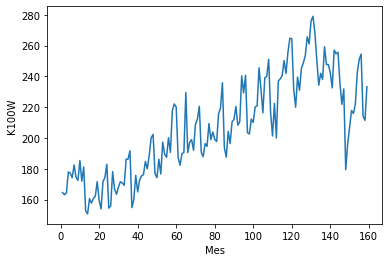
\includegraphics[width=\columnwidth]{fig_1}
\caption{Valor de K100W por mes}
\label{fig:1}
\end{figure}

Al aplicar el ajuste polinomial sobre estos datos, se obtuvo el polinomio $K(m)=c_1m^8+c_2m^7+c_3m^6+c_4m^5+c_5m^4+c_6m^3+c_7m^2+c_8m+c_9$, donde $m$ corresponde al mes (tomando enero del 2008 como $m=0$) y los valores de las constantes $c_i$ son:

$$c_1=1.0941010488289785\times10^{-13}$$
$$c_2=-4.53860066817757\times10^{-11}$$
$$c_3=5.0133104673499385\times10^{-9}$$
$$c_4=2.830105232161398\times10^{-7}$$
$$c_5=-9.519874506850869\times10^{-5}$$
$$c_6=0.006778658362009159$$
$$c_7=-0.17439399870456623$$
$$c_8=1.3650936871410662$$
$$c_9=168.13043624937725$$

\medskip

En la figura \ref{fig:2} se muestra la gráfica de $K(m)$ comparada con los datos. Como se puede apreciar, la diferencia entre los datos y el valor del polinomio de ajuste es en ocasiones muy elevada; para facilitar su visualización, en la figura \ref{fig:3} se muestra el valor porcentual de dicha diferencia para cada mes.

\begin{figure}[h]
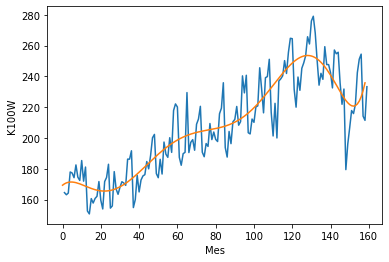
\includegraphics[width=\columnwidth]{fig_2}
\caption{Función de ajuste polinomial}
\label{fig:2}
\end{figure}

\begin{figure}[h]
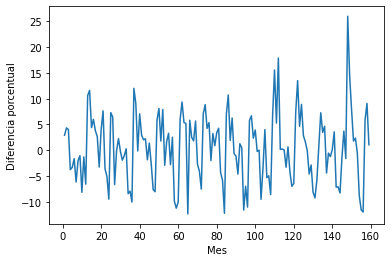
\includegraphics[width=\columnwidth]{fig_3}
\caption{Diferencia porcentual entre el valor de K100W y el polinomio obtenido del ajuste}
\label{fig:3}
\end{figure}

\medskip

Como paso final, se calculó el valor de la proyección $K(m)$ para los meses de abril a diciembre de 2021 (correspondientes los valores de $m=160$ a $m=168$ conforme al convenio de numeración establecido previamente). Los valores obtenidos son:

$$K(160) =  242.33920300882275$$
$$K(161) =  250.4613596106305$$
$$K(162) =  260.3502615256044$$
$$K(163) =  272.2097116573258$$
$$K(164) =  286.2586105744232$$
$$K(165) =  302.7317118841941$$
$$K(166) =  321.88040253547524$$
$$K(167) =  343.97350854225056$$
$$K(168) =  369.29812662535005$$

cuya gráfica se muestra en la figura \ref{fig:4}.

\begin{figure}[h]
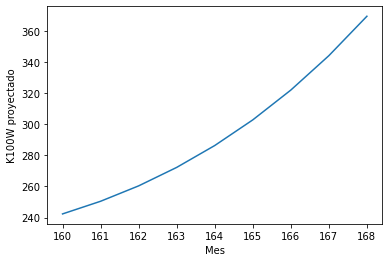
\includegraphics[width=\columnwidth]{fig_4}
\caption{Valores proyectados de K100W para los meses 160-168}
\label{fig:4}
\end{figure}

\section{Fe de erratas}

En la presentación de lunes 14 de junio, se presentaron datos que cubrían 318 meses. Eso es \textbf{incorrecto}, el error procede de no haber considerado el desglose de los datos mensuales en comercio al por mayor y al por menor, como se detalla en la sección 2.

\end{document}
